\chapter{Geladenes Teilchen im elektrischen Feld\label{chapter:efeld}}
\lhead{Teilchen im elektrischen Feld}
\begin{refsection}
\chapterauthor{Michael Cerny und Stefan Schindler}


In diesem Kapitel erweitern wir das Beispiel des Potentialkastens 
(Kapitel \ref{subsection:potentialkasten}, Seite \pageref{subsection:potentialkasten})
um eine St\"orung.

\section{Formeln der St"orungstheorie}
Grunds"atzlich k"onnen wir mit der St\"orungstheorie ein einfaches Modell 
(Abb \ref{abb:efeld_psi_ungestoert} der ersten 5 Energieniveaus) 
mit einer St\"orung erg"anzen, statt von Anfang an mit einem komplexen Modell zu rechnen.

Allgemein gilt:
\[
  f(x, \varepsilon) = f_0(x) + \varepsilon f_1(x) + \varepsilon^2 f_2(x) + \ldots + \varepsilon^n f_n(x)
\]
Dabei ist $f_0(x)$ die urspr\"ungliche Funktion und $f_n(x)$ die $n$-te  N"aherung der St"orung.
Mit $\varepsilon$ wird die St"orung gesteuert. Dabei sollte $\varepsilon$ nicht zu gross gew"ahlt werden, 
da die N"aherung sonst ungenau wird. 

Setzen wir $\varepsilon = 0$, k\"onnen wir die St"orung dynamisch abschalten.

In der Quantenmechanik k"onnen wir die St"orungstheorie anwenden indem wir den Hamilton-Operator der 
urspr"unglichen Funktion $H_0$ um zus"atzliche $\varepsilon^n H_n$ erg"anzen:
\[
  H = \varepsilon^0 H_0 + \varepsilon^1 H_1 + \varepsilon^2 H_2 + \ldots + \varepsilon^n \hat H_n
\]



\begin{figure}
 \centering
 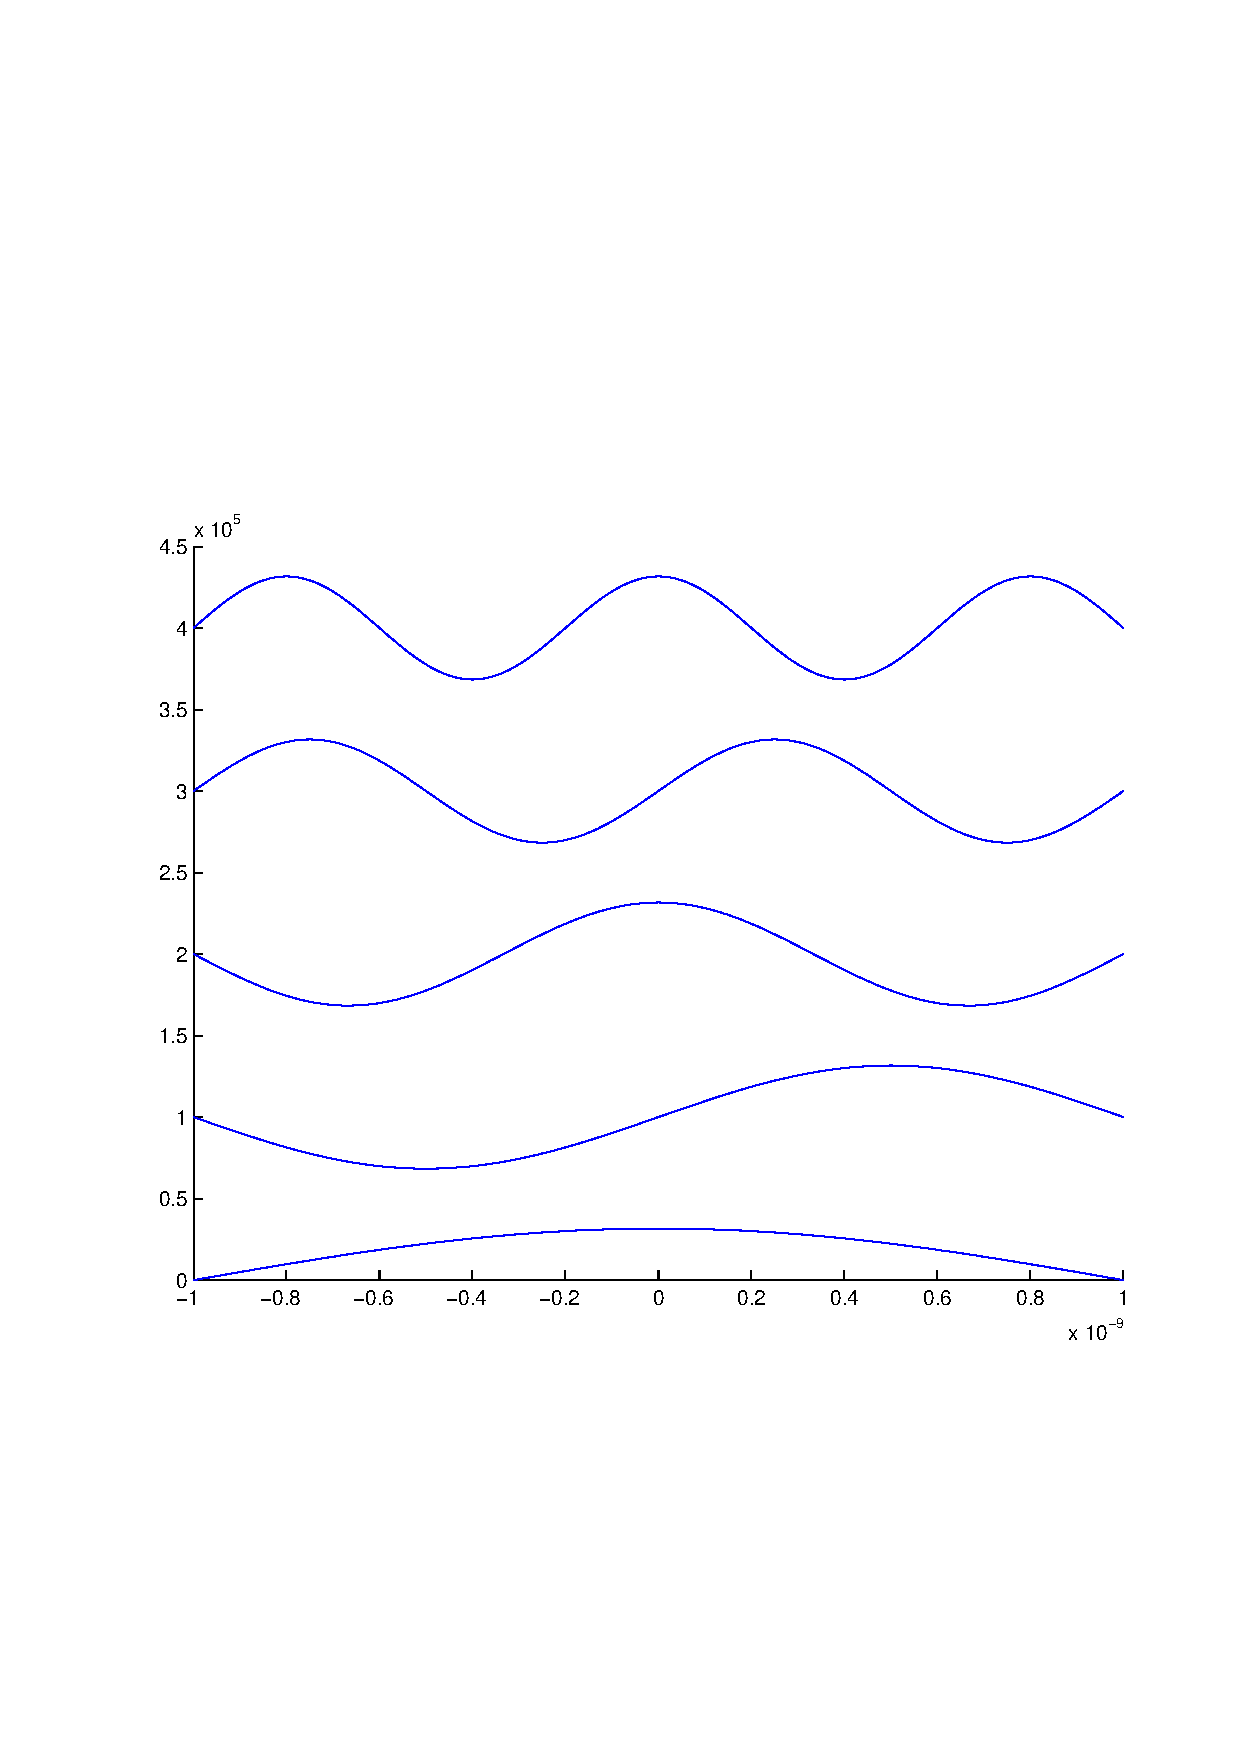
\includegraphics[width=12cm,clip=true,trim=2cm 7cm 1cm 8cm]{efeld/Psi_ungestoert.pdf}
 \caption{$\psi$ ungest\"ort}
 \label{abb:efeld_psi_ungestoert}
\end{figure}












\section{Potentialkasten mit elektrischem Feld}

\subsection{Ausgangslage}

Bei unserer Anwendung bauen wir auf dem Potentialkasten 
(Kapitel \ref{subsection:potentialkasten}, Seite \pageref{subsection:potentialkasten}) auf.

Dabei geht es um ein Elektron welches zwischen zwei Barrieren mit unendlich hohem Potential gefangen ist.
Zwischen den Barrieren kann sich das Teilchen mit den Wellenfunktionen $\psi_k$ bewegen,
ausserhalb kommt es hingegen nicht vor.

Wir erweitern jetzt das System mit einer St"orung, indem wir eine elektrische Spannung anlegen.
Weil das Elektron eine negative Ladung besitzt ver"andert sich seine Wellenfunktion.

Als Grundlage "ubernehmen wir zwei Funktionen aus dem Skript
\begin{equation}
\begin{aligned}
H^{(0)}&=\frac1{2m}p^2+V^{(0)}(x)
\\
V^{(0)}(x)&=
  \begin{cases}
    0       & \qquad |x|<l\\
    \infty  & \qquad\text{sonst}
  \end{cases}
\end{aligned}
\end{equation}

und erweitern sie mit der St"orung $V^{(1)}$, welche wir als lineares Feld definieren:
% FIXME Link pr\"ufen
\begin{equation}
  \label{eq:efeld_v0_kasten}
  V^{(1)}(x) = a x + b
\end{equation}

Die St"orung kann noch weiter vereinfacht werden:

Da wir $a$ bereits durch $\varepsilon$ beschreiben, k\"onnen wir mit $a = 1$ vereinfachen,
und weil die Barrieren unendlich hoch sind, k"onnen wir $b = 0$ setzen.

Wenn wir jetzt die St"orung einsetzen, bekommen wir die neue Hamilton-Funktion
\[
  H=\frac1{2m}p^2+V^{(0)}(x)
    + \varepsilon x.
\]
aus welcher wir den Hamilton-Operator berechnen k"onnen:
\[
  \hat{H} = -\frac{\hbar^2}{2m} \frac{\partial^2}{\partial x^2} + V^{(0)}(x) + \varepsilon x
\]

\subsection{Vorgehensweise}
Wir berechnen in unserem Beispiel die erste N"aherung.

Im Kapitel \ref{skript:stoerungsloesung1ordnung} wird beschrieben wie man von der Schr"odingergleichung 
auf die erste N"aherung kommt.

Entscheidend hier ist ob die Zust"ande entartet sind oder nicht.
Entartung bedeutet, dass zwei Zust"ande die selbe Energie besitzen, wodurch der Nenner zu Null wird.
Das w"are der Fall wenn das Elektron aus dem Kasten entkommen w"urde,
dann h"atten zwei Wellen ausserhalb des Kastens die selbe Energie.

Diesen Fall schliessen wir mit den unendlich hohen Barrieren aus.

Wir benutzen also folgende Funktionen
\begin{equation}
\begin{aligned}
E_k^{(1)} &=
\langle \psi_k^{(0)}|\, H_1 \,|\psi_k^{(0)}\rangle
\\
|\psi_k(\varepsilon)\rangle &=
(1+i\varepsilon \gamma)
\,|\psi_k^{(0)}\rangle
+
\varepsilon
\sum_{k\ne l}
\frac{\langle \psi_l^{(0)}|\, H_1 \,|\psi_k^{(0)}\rangle}{E_k^{(0)}-E_l^{(0)}}
\,
|\psi_l^{(0)}\rangle
\end{aligned}
\end{equation}









\subsection{Berechnung des Modells mit MATLAB}

Ausserdem ist das urspr"unglich $Psi_k^{(0)}$ gegeben.

Um jetzt das gest"orte System zu berechnen brauchen grunds"atzlich nur drei Formeln:
\begin{equation}
\begin{aligned}
k&=l
&&\Rightarrow&
E_k^{(1)}
&=
\langle \psi_k^{(0)}|\, H_1 \,|\psi_k^{(0)}\rangle
\\
k&\ne l
&&\Rightarrow&
\langle\psi_l^{(0)}|\psi_k^{(1)}\rangle
&=
\frac{\langle \psi_l^{(0)}|\, H_1 \,|\psi_k^{(0)}\rangle}{E_k^{(0)}-E_l^{(0)}}
\end{aligned}
\end{equation}

\begin{equation}
|\psi_k(\varepsilon)\rangle
=
(1+i\varepsilon \gamma)
\,|\psi_k^{(0)}\rangle
+
\varepsilon
\sum_{k\ne l}
\frac{\langle \psi_l^{(0)}|\, H_1 \,|\psi_k^{(0)}\rangle}{E_k^{(0)}-E_l^{(0)}}
\,
|\psi_l^{(0)}\rangle
\end{equation}

Mit der ersten Gleichung k"onnen wir direkt die Energie der St"orung berechnen.

Man berechnet das Skalarprodukt $\psi_k^{(0)}$ und $x \psi_k^{(0)}$ "uber 
die gesamte L"ange des Potenzialkastens und erh"alt so $E_k^{(1)}$.

So k\"onnen wir die aufsummierte Energie mit $E_k^{(0)} + \varepsilon E_k^{(1)}$ berechnen.

\begin{lstlisting}[style=Matlab]
...
H1 = x;
for k = 1 : 5
  E1(k) = dot(Psi(k, :), H1.*Psi(k, :));
  plot(epsilon, E0(k) + epsilon*E1_k(k))
end
\end{lstlisting}
In Psi befinden $k$ Vektoren mit diskreten Abtastwerten von $\psi^{(0)}$ \"uber die die L\"ange $2l$
\& mit $Psi(k, :)$ ausgelesen werden.

Das Resultat sehen wir in der Abbildung \ref{abb:efeld_E_gestoert}.

Um $\psi_k(\varepsilon)$ zu berechnen wird es etwas schwieriger, weil sich in der Quantenmechanik die Energiezust"ande $k$ gegenseitig beeinflussen.

Daher setzen wir eine St"orung $\psi_k^{(1)}$ aus mehreren $\psi_k^{(0)}$ zusammen.
Mit der zweiten und dritten Formel k"onnen wir diesen Anteil berechnen.

\begin{equation}
  \label{eq:efeld_skalar_gleichung}
  \langle\psi_l^{(0)}|\psi_k^{(1)}\rangle
      =
  \frac{\langle \psi_l^{(0)}|\, H_1 \,|\psi_k^{(0)}\rangle}{E_k^{(0)}-E_l^{(0)}}
\end{equation}

Die Formel \ref{eq:efeld_skalar_gleichung} ergibt einen Skalarwert, welchen Anteil die Welle $l$ an der St"orung $k$ hat.

Um zum Beispiel den f"unften Zustand $\psi_5^{(1)}$ zu bestimmen addieren wir alle 
$\langle\psi_l^{(0)}|\psi_5^{(1)}\rangle|\psi_l^{(0)}\rangle$
 von 1 bis n ausser 5.
\begin{equation}
  \sum_{l=1 ; l\ne 5}^{\infty}
    \frac{\langle \psi_l^{(0)}|\, H_1 \,|\psi_k^{(0)}\rangle}{E_k^{(0)}-E_l^{(0)}}
        \,
    |\psi_l^{(0)}\rangle
\end{equation}

In Matlab wird das wie folgt implementiert:
\begin{lstlisting}[style=Matlab]
...
L = -10^-9;           # Breite des Potentialkastens
x = -L : delta : L;   # Bereich definieren
H1 = x;               
n = 1000;             # Anzahl aufsummierte Zust\"ande
k = 5;                # Anzahl geplotete Zust\"ande
summe = 0;
for l = 1 : n
  if l ~= k           # Vergleich l != k
    Psi0_l = dot(Psi(l, :), H1.*Psi(k, :)) / (E(k)-E(l)) .* Psi(l, :);
    summe = psi1_l + psi0_l;
  end
end
\end{lstlisting} % FIXME Summe

Man muss zum Gl"uck nicht unendlich viele Zahlen addieren, da der Anteil wegen $\frac{1}{E(k)-E(l)}$ immer weiter abnimmt.
In diesem Fall addieren wir bei $l=90$ nur $1\%$ der St"orung dazu, bei $l=280$ nur noch $0.1\%$.

Wir k"onnen jetzt die St"orung in 
\begin{equation}
|\psi_k(\varepsilon)\rangle
=
(1+i\varepsilon \gamma)
\,|\psi_k^{(0)}\rangle
+
\varepsilon|\psi_k^{(1)}\rangle
\end{equation}
einsetzen und bekommen so die neue Wellenfunktion die man in \ref{abb:efeld_psi_gestoert} sehen kann.

\subsection{Auswertung Psi}

\begin{figure}
 \centering
 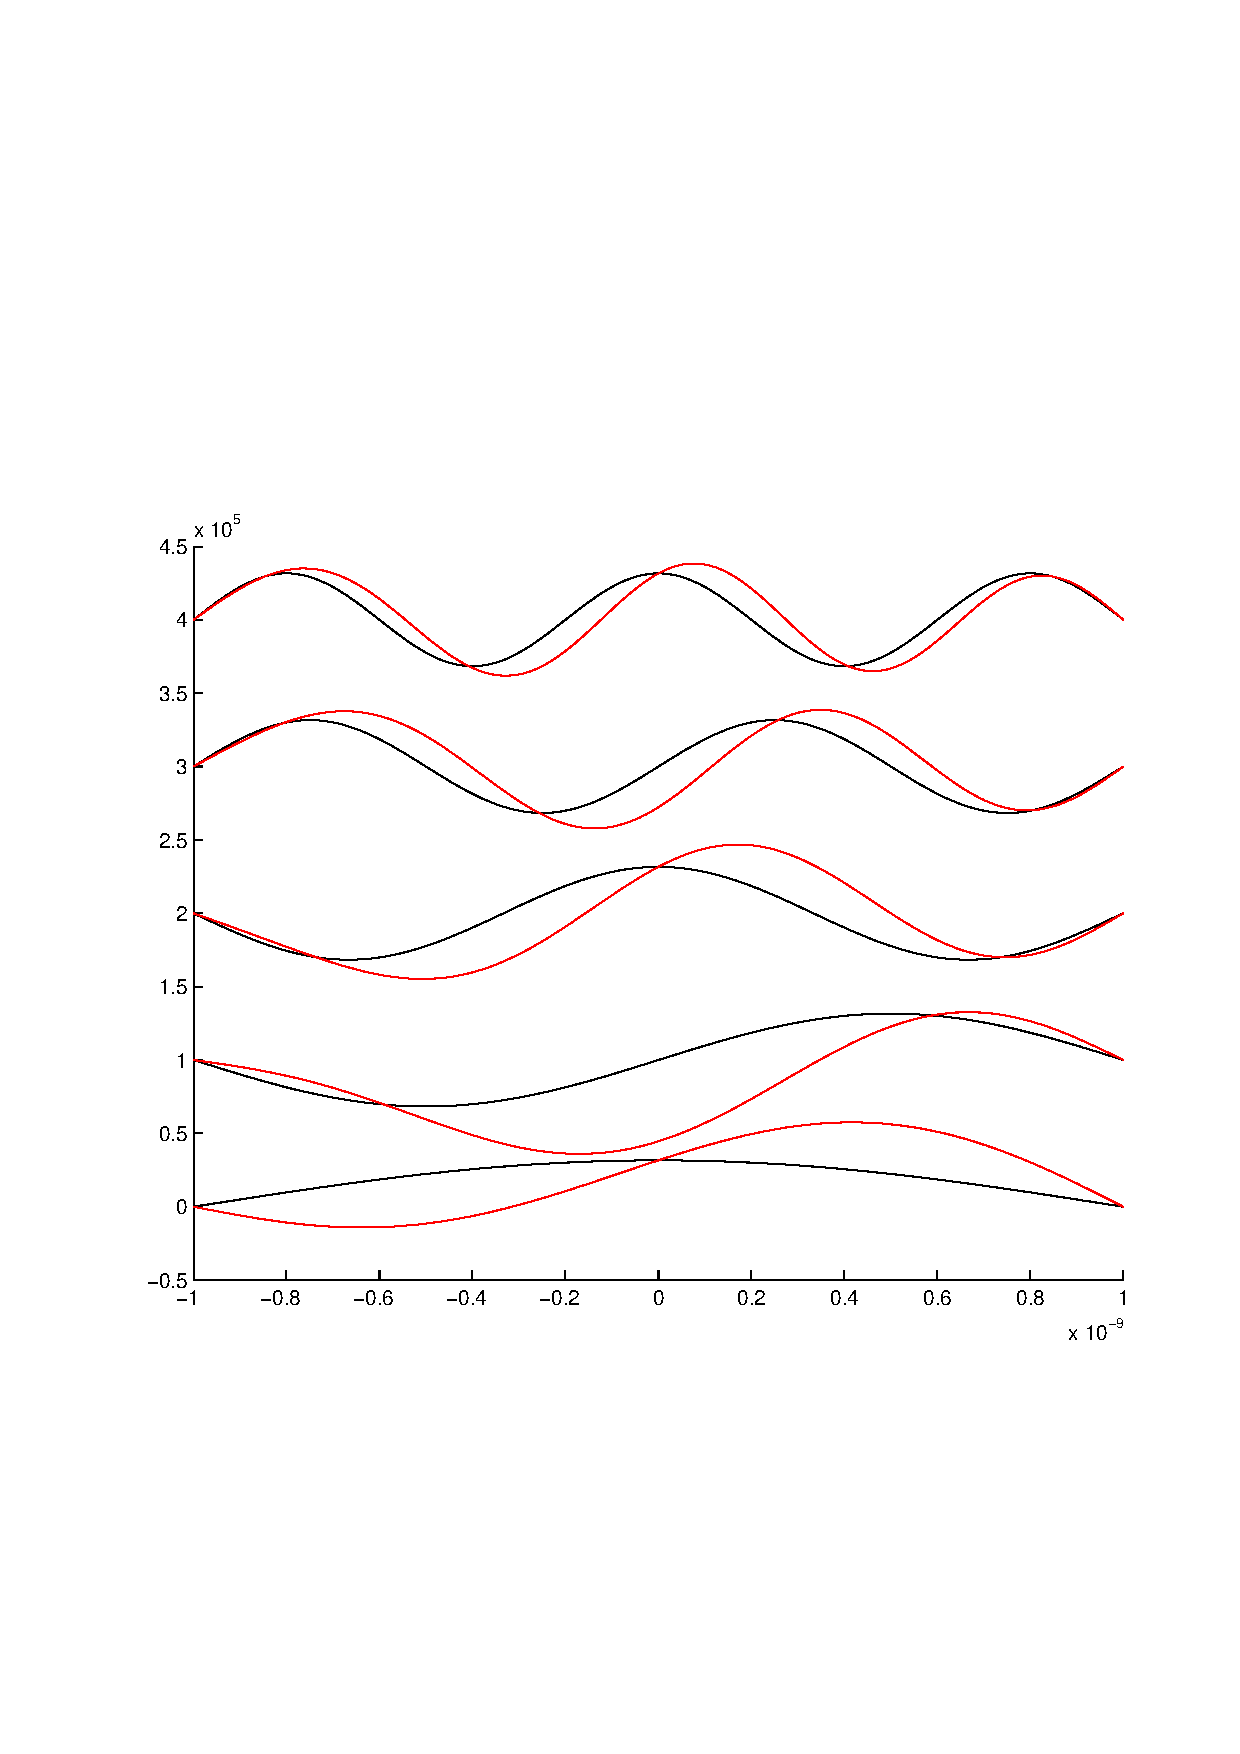
\includegraphics[width=12cm,clip=true,trim=2cm 7cm 1cm 8cm]{efeld/Psi_gestoert.pdf}
 \caption{$\psi$ gest\"ort}
 \label{abb:efeld_psi_gestoert}
\end{figure}

In der Grafik \ref{abb:efeld_psi_gestoert} sehen wir die Unterschiede zwischen dem normalen $\psi$ (schwarz) 
\& der ersten N"aherung (rot).


Auf der vertikalen Achse haben wir die Amplituden von $\psi_k$.
$\psi^2$ entspricht der Wahrscheinlichkeitsdichte das sich das Elektron an dieser Stelle befindet.
Die Werte der Kurven pendeln um Null \& wurden nur der Lesbarkeit halber getrennt.

Auf der Horizontalen sehen wir die x-Position vom Teilchen im zweidimensionalen Potentialkasten.

Subjektiv betrachtet sieht es aus als sei die Wellenfunktion nach links gedr"uckt.
Das kommt daher dass das Elektron auf der gesamten L"ange die selbe Energie haben muss,
denn sonst m"uste es sie ja auf dem Weg aufnehmen (die Gesamtenergie kann sich hingegen mit der St"orung ver"andern).

Weil wir jetzt aber ein elektrisches Feld angelegt haben, hat das Elektron auf der rechten Seite ein h"oheres Potential.

Wie der Ausgleich funktioniert, kann man in der Schr"odingergleichung 
$
-\frac{\hbar^2}{2m}\Delta\Psi(x) + V(x)\Psi(x)
=
E\Psi(x)
$ sehen
Weil $E\Psi(x)$ konstant ist, sinkt bei einem h"oherem Potential $-\frac{\hbar^2}{2m}\Delta\Psi(x)$,
was einer Abnahme der Frequenz entspricht.



Wir haben in dieser Abbildung das Epsilon sehr stark gew"ahlt,
weil bei einem schwachen Epsilon die "Anderungen nur schlecht sichtbar sind.







In diesem Beispiel haben wir die Unterschiede mit sehr starken Parametern gew"ahlt.




\subsection{Auswertung E}

In der Grafik \ref{abb:efeld_E_gestoert} lassen wir f"ur die jeweiligen stabilen Zust"ande 0..4 
den Einfluss der St"orung wachsen.

Da das elektrische Feld jedoch nur einen sehr kleinen Einfluss auf die gesamte Energie des 
Elektrons hat, mussten wir um die Effekte der 1. N"aherung zu zeigen ein sehr grosses $\varepsilon$
w"ahlen.

\begin{figure}
 \centering
 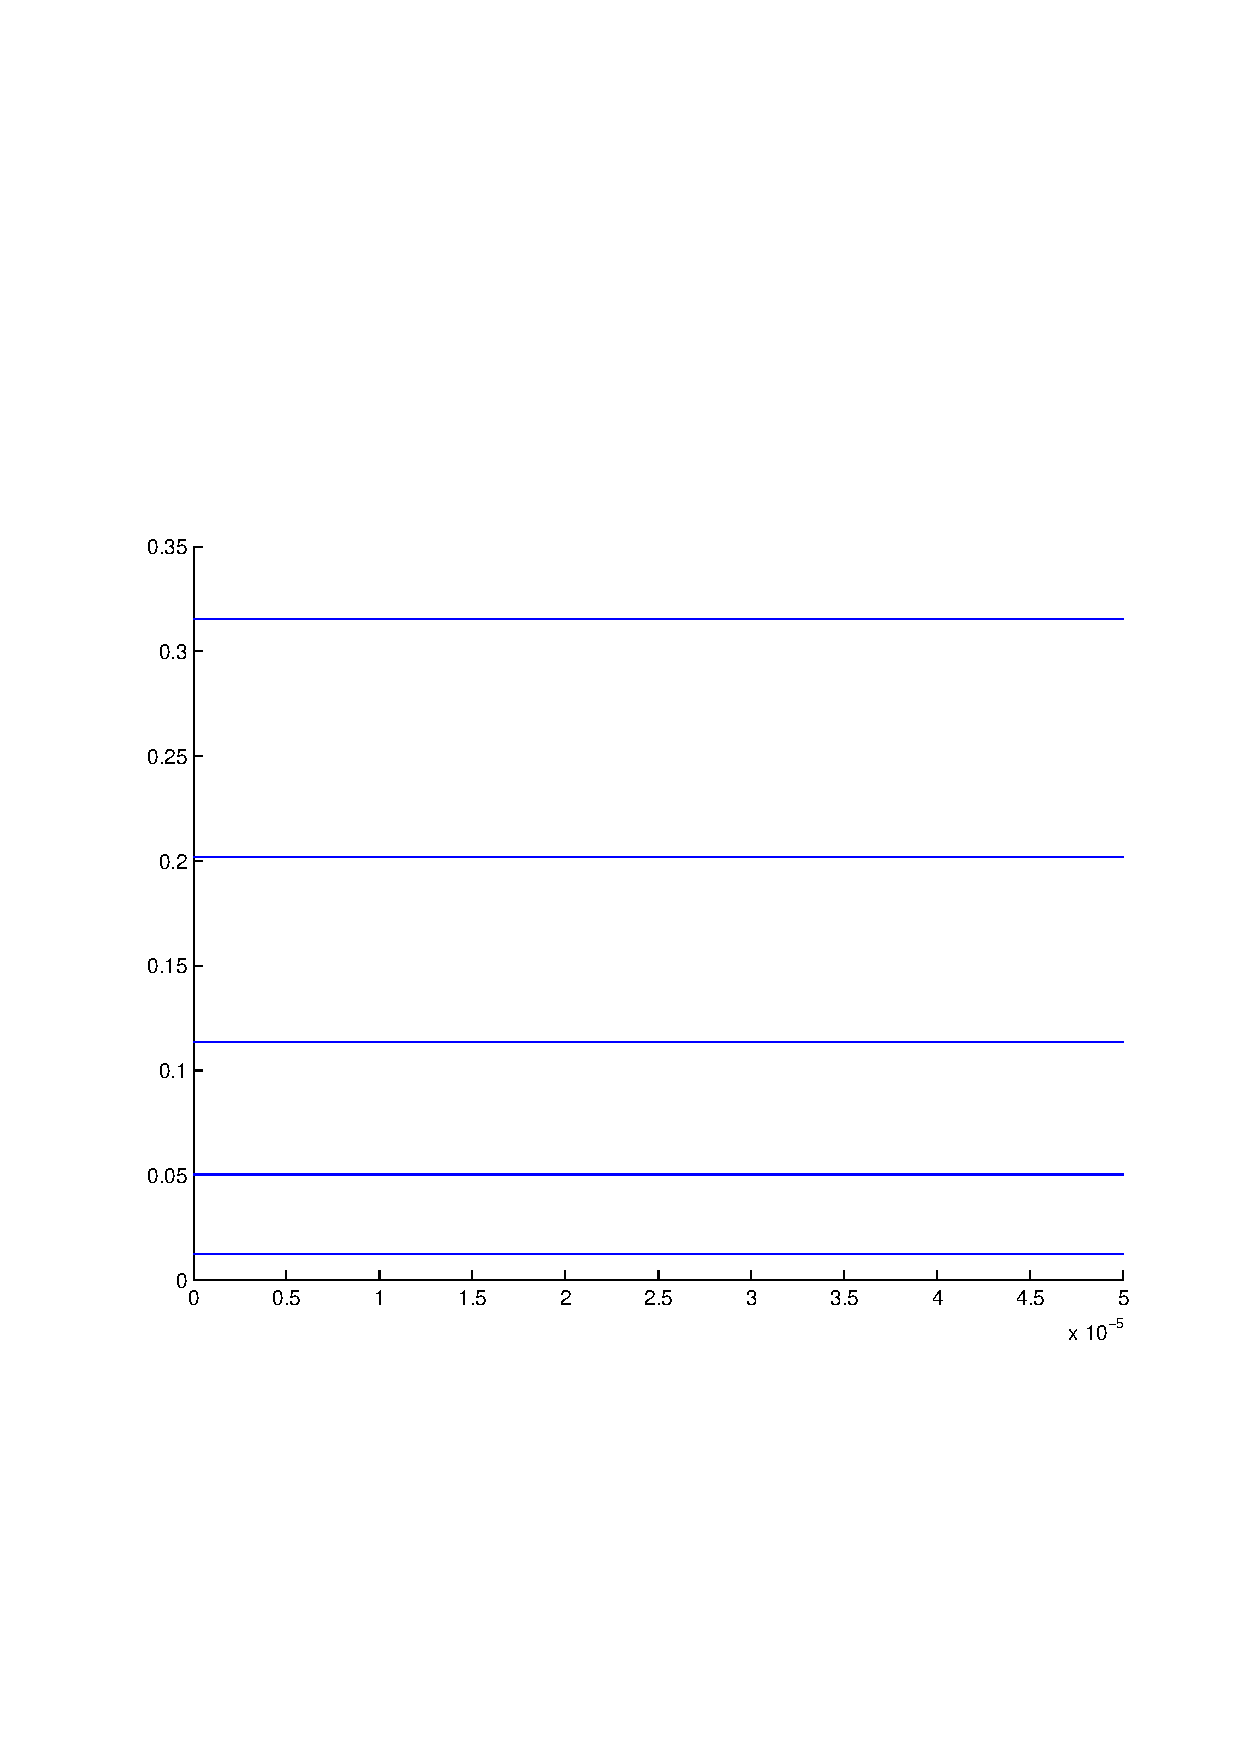
\includegraphics[width=12cm,clip=true,trim=2cm 7cm 1cm 8cm]{efeld/Energie_gestoert.pdf}
 \caption{$E$ gest\"ort, horizontale Achse ist $\varepsilon$, vertikale Achse ist die gesammte Energie des Systems}
 \label{abb:efeld_E_gestoert}
\end{figure}







\printbibliography[heading=subbibliography]
\end{refsection}
